\documentclass[times, utf8, zavrsni]{fer}
\usepackage{booktabs}
\graphicspath{ {./images/} }
\setcitestyle{numbers,square,unsrt}

\begin{document}

\thesisnumber{1003}

\title{Prevoditelj za novi programski jezik}

\author{Lana Šprajc}

% \maketitle

% Ispis stranice s napomenom o umetanju izvornika rada. Uklonite naredbu \izvornik ako želite izbaciti tu stranicu.
%\izvornik

% Dodavanje zahvale ili prazne stranice. Ako ne želite dodati zahvalu, naredbu ostavite radi prazne stranice.
\zahvala{}

\tableofcontents

\chapter{Uvod}
Postoji velik broj programskih jezika. Svaki od njih ima neke prednosti i mane te svoje namjene.
Neki jezici se prevode u jako vremenski i prostorno efikasan kod, no ti jezici u većini slučajeva imaju strmu krivulju učenja. Početnici u ovakvim jezicima
rade puno grešaka i često odustaju od učenja jezika. Primjeri ovakvih jezika su C i C++. S druge strane, puno jezika ima jednostavnu sintaksu, sličnu pseudokodu, ali
često su neefikasni. Primjer ovakvog jezika je Python.

Cilj ovog rada je napraviti jezik koji je jednostavan za korištenje i učenje, a koji se prevodi u efikasan kod.

Rad je podijeljen u 9 poglavlja. U drugom poglavlju su opisani osnovni dijelovi programskih jezika i neke specifičnosti koje su dozvoljene u određenim jezicima.
U trećem poglavlju je opisana arhitektura prevoditelja programskih jezika. U četvrtom poglavlju je opisana sintaksa novog programskog jezika L\#. U petom poglavlju
je sintaksa formalizirana pomoću gramatike jezika. U šestom poglavlju je opisan način rada razvijenog prevoditelja. U sedmom poglavlju su dane upute za instalaciju
i pokretanje prevoditelja. Osmo poglavlje daje prikaz primjera ulaznih i izlaznih datoteka. U devetom poglavlju iznesen je zaključak.

\chapter{Osnovni dijelovi programskih jezika}
Glavni dijelovi programskog koda u gotovo svim programskim jezicima su klase, funkcije, naredbe i varijable. Slijedi kratki pregled svakog od tih dijelova.

\section{Varijable i tipovi podataka}
Varijable su spremnici vrijednosti.

Svaki podatak spremljen u varijablu ima neki tip. Tipovi se dijeli na brojeve (cijele i decimalne), stringove, polja i tipove definirane od strane korisnika. Posljednje
čine klase (engl. \textit{class}) u objektno orijentiranim jezicima (C++, Java, Python...) i strukture (engl. \textit{struct}) u C-u.

\subsection{Statički i dinamički tipizirani jezici}
S obzirom na pristup varijablama, jezici mogu biti statičkih tipova (engl. \textit{staticly typed}) i dinamičkih tipova (engl. \textit{dinamicly typed}).
Jezici statičkih tipova provjeravaju tip podatka tijekom kompilacije zbog čega se ne događaju pogreške prilikom izvođenja koda. U jezicima statičkih tipova, nije moguća promjena tipa 
varijable kroz kod \citep{pythonplanet}. Primjeri statičkih tipiziranih jezika su C, C++, Java\dots

Jezici dinamičkih tipova provjeravaju tip tijekom izvođenja (engl. \textit{runtime}). Ovo usporava rad prevedenog programa jer se tijekom izvođenja koda mora provoditi provjera tipova \citep{pythonplanet}.
Primjeri dinamički tipiziranih jezika su Python, Javascript\dots

\subsection{Slabo i jako tipizirani jezici}
Jezici se dijele slabo tipizirane (engl. \textit{weakly typed}) i jako tipizirane (engl. \textit{strongly typed}). Iako ne postoji općeprihvaćena definicija, 
najčešća interpretacija je da ovo označava u kojoj mjeri jezici podržavaju implicitne konverzije iz tipa u tip i operacije različitih tipova. Jezici koji podržavaju ovo nazivaju
se slabo tipizirani, dok se jezici koji ne podržavaju zovu jako tipizirani. Važno je napomenuti da se radi o skali, a ne strogoj podjeli. Tako je primjerice Python jače tipizirani od JavaScripta \citep{zolatypes}. 

\section{Naredbe}
Naredbe su osnovni dio programskog koda. Osnovne naredba su naredbe deklaracije, naredbe pridruživanja, naredbe grananja, naredbe petlja i naredbe poziva funkcije.

\section{Funkcije}
Funkcije su odvojeni dijelovi koda koji se izvršavaju prilikom poziva. Funkcija ima svoju deklaraciju i definiciju. Deklaracija se sastoji od imena funkcije, povratne vrijednosti 
te niza argumenata koje funkcija prima. U definiciji funkcije nalaze se i naredbe koje se izvršavaju prilikom poziva funkcije. U nekim jezicima argumenti funkcije mogu imati 
pretpostavljene (engl. \textit{default}) vrijednosti (npr. Python), ali ovo nije moguće u svim jezicima (npr. C).

\subsection{Preopterećene funkcije}
Preopterećivanje funkcija (engl. \textit{function overload}) je stvaranje funkcija s jednakim imenom, a različitim argumentima. Argumenti se mogu razlikovati po tipovima
ili po broju. Neki jezici koji ovo podržavaju su C++, Java, Julia \citep{Kahanwal2014ComparativeSO}, dok preopterećene funkcije nisu moguće u C-u, Pythonu\dots Većina dinamički tipiziranih jezika ne podržava
preopterećene funkcije jer prilikom prevođenja koda nije poznata informacija o tipu argumenata pa prevoditelj ne može donijeti odluku o pozivu ispravne funkcije.

\section{Klase}
Klase su dio svih objektno orijentiranih jezika. One predstavljaju definiciju novih vrsta podataka koje se sastoje od članova (drugih varijabli) te metoda (funkcija koje se pozivaju
nad instancom klase i najčešće joj mijenjaju vrijednost). Instanca klase naziva se objekt.

\chapter{Prevoditelji programskih jezika}
Prevoditelji programskih jezika su programi koji kod napisan u zadanom programskom jeziku pretvaraju u drugi programski jezik (najčešće niže razine) i pritom provjeravaju njegovu ispravnost.
Postupak prevođenja programskog jezika ugrubo se dijeli na analizu izvornog programa i sintezu zadanog programa. Najčešći dijelovi prevoditelja programskih jezika su leksička analiza,
sintaksna analiza, semantička analiza, generiranje ciljnog programa te optimizacija ciljnog programa.

\section{Kompajler i interpreter}
Prevoditelji programskih jezika se dijele na kompajlere i interpretere. Kompajleri prije pokretanja programa prevedu i spreme sav kod, dok interpreteri 
prevode kod za vrijeme izvršavanja programa \citep{compilerint}. 

\section{Leksička analiza}
Leksička analiza čini prvi dio analize izvornog programa. Cilj leksičke analize je dobivanje niza tokena koji predstavljaju glavne dijelove programa \citep{ppj}. 

\subsection{Token}
Token predstavlja najmanju cjelinu u izvornom programu. Tokeni se dijele na ključne riječi, varijable, konstante, operatore i posebne znakove (npr. zagrade, točka zarez, zarez, dvotočka).
Za svaki token, leksički analizator sprema vrijednost, tip i liniju u kojoj se pojavljuje. Vrijednost i tip se koriste u sljedećim dijelovima analize dok se linija čuva kako bi se u slučaju pogreške mogla
dati opširnija informacija o mjestu pogreške.

\subsection{Način rada leksičkog analizatora}
Leksički analizator (tokenizator, lekser) je konačni automat koji prolazi znak po znak kroz izvorni kod. Miče znakove praznine (engl. \textit{whitespace characters}) kao što su razmaci,
tabulatori, i prelazi u različita stanja na temelju pročitanih znakova.
Kada uđe u konačno stanje, npr. čitanjem praznine ili operatora, lekser generira token \citep{ppj}. 

\section{Sintaksna analiza}
Sintaksna analiza je središnji dio prevođenja programskog jezika. Za potrebe sintaksne analize gradi se gramatika jezika prema kojoj sintaksni analizator analizira (parsira) izvorni kod.
Zadaci sintaksnog analizatora su provjera sintaksnih pravila, određivanje mjesta sintaksnih pogrešaka i gradnja sintaksnog stabla \citep{ppj}.  Sintaksna analiza se dijeli na analizu od dna prema vrhu (engl. \textit{bottom up}) i od vrha prema dnu (engl. \textit{top down}). Tijekom sintaksne analize se također stvaraju zapisi o svakoj varijabli, funkciji, klasi \dots

\subsection{Sintaksno stablo}
\begin{figure}
    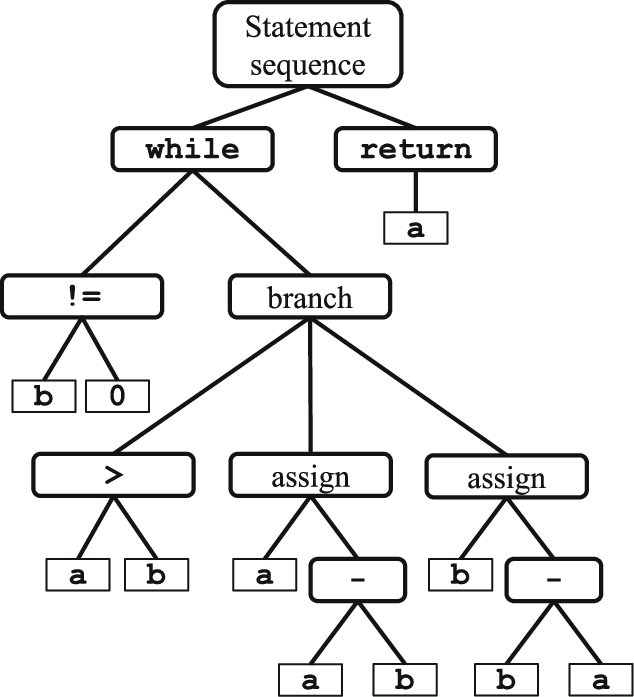
\includegraphics[scale=0.5]{800px-Abstract_syntax_tree_for_Euclidean_algorithm.svg.png}\\
    \caption{Primjer sintaksnog stabla \citep{slika}}
\end{figure}

Sintaksno stablo je rezultat sintaksne analize. Čvorove sintaksnog stabla čine glavni strukturalni dijelovi programskog koda, kao što su naredbe grananja,
izrazi\dots Na slici 3.1 je prikazan primjer sintaksnog stabla izgrađenog nad sljedećim pseudokodom.
\begin{verbatim}
    while (b != 0) {
        if (a > b)
            a = a - b
        else
            b = b - a
    }
    return a
\end{verbatim}

\pagebreak
\subsection{Analiza od vrha prema dnu i od dna prema vrhu}
Sintaksni analizator može graditi sintaksno stablo od vrha prema dnu ili od dna prema vrhu.

\subsubsection{Gradnja stabla od vrha prema dnu}
Gradnju stabla od vrha prema dnu, sintaksni analizator započinje u vršnom čvoru. U svakom koraku, na temelju 
pročitanih tokena i čvora u kojem se nalazi, analizator ili stvara novi čvor niže razine i prelazi u njega ili završava čvor u kojem se nalazi
i vraća se u roditeljski čvor. Sintaksni analizator može graditi stablo od vrha prema dnu na temelju S-gramatike,
Q-gramatike i LL(1)-gramatike \citep{ppj}. 

\subsubsection{Gradnja stabla od dna prema vrhu}
Prilikom gradnje stabla od dna vrema vrhu, sintaksni analizator čita token po token te ih pokušava spojiti u zajednički vršni čvor.
Kada izgradi čvor pokušava taj čvor spojiti u viši čvor sa sljedećim tokenima ili čvorovima sve dok ne dođe do vrha stabla.
Ovo je moguće pomoću tehnika pronađi-pomakni, pronađi-reduciraj, tehnikom prednosti operatora i pomoću LR parsiranja \citep{ppj}. 

\section{Semantička analiza}
Postupkom semantičke analize, čvorovima sintaksnog stabla se određuju semantička svojstva, pronalaze se semantičke pogreške
te se semantička svojstva prosljeđuju \linebreak s čvora na čvor stabla \citep{ppj}. Semantička svojstva uključuju tip podatka, vrijednost izraza\dots

\section{Generiranje koda}
Na temelju prethodnih koraka, prevoditelj programskog jezika generira ciljni kod. U ovom trenutku prevoditelju je poznato
kojeg su tipa sve varijable, njihova ime i početne vrijednosti (ako ih imaju), na kojem su mjestu sve naredbe, popis svih funkcija i naredba koje se trebaju izvršavati u njima \dots
Iz ovih podataka, prevoditelj generira ekvivalentne izraze u ciljnom jeziku i time stvara ciljni program \citep{ppj}. 

\section{Optimizacija}
U generiranom kodu mogu se pojaviti operacije koje samo usporavaju rad programa. Primjerice pridruživanje vrijednosti varijabli koja se nakon toga ne koristi
ili generiranje 2 do 3 izraza koji se mogu spojiti u jedan.
Cilj postupka optimizacije je micanje ovakvih izraza kako bi generirani kod bio što brži i koristio što manje memorije.

\chapter{Sintaksa jezika L\# }
U sklopu ovog rada osmišljen je novi programski jezik L\# (ekstenzija .l). Sastoji se od varijabli (cjelobrojnih, decimalnih, stringova, polja), 
funkcija i klasa. Nije moguće preopterećivanje funkcija. Varijable su statički tipizirane.

\section{Komentari}
Komentari započinju znakom \verb|#| te se protežu do kraja reda. Nije moguće 
stvoriti jedan komentar koji se proteže kroz više redova.

\section{Varijable}
Sva imena varijabli započinju slovom i sastoje se od slova, brojeva i znaka \_. Moguće je definirati varijablu implicitno joj zadajući tip, primjerice korištenjem
izraza \verb|lana = 3;| ili eksplicitno, primjerice korištenjem izraza \verb|lana = int8;|. U prvom slučaju varijabli se zadaje jednak tip kao što ima izraz
koji joj se pridružuje.

Osnovni tipovi varijabla su \verb|bool|, 
\verb|int8|,  \verb|int16|,  \verb|int32|,  \verb|int64|, 
\verb|uint8|, \linebreak  \verb|uint16|,  \verb|uint32|,  \verb|uint64|, 
\verb|float32|,  \verb|float64|,  \verb|float96| i \verb|string|

\subsection{Polja}
Polja se u jeziku L\# definiraju dodavanjem znakova \verb|[| i \verb|]| iza tipa varijable. Nije moguće implicitno zadati tip polja tako da mu se zadaje vrijednost.
Elementu polja pristupa se indeksom između znakova \verb|[ ]|. Polja su indeksirana od nule.

\section{Funkcije}
Sav kod (osim definicija globalnih varijable i klasi) nalazi se unutar funkcija. Slijedi pregled načina definiranja i pozivanja funkcija.
\subsection{Definicija funkcije}
Definicija funkcije, sastoji se od imena funkcije, zagrada unutar kojih se nalazi popis argumenata. Za svaki argument je potrebno eksplicitno navesti tip. Nije moguće 
postavljanje pretpostavljene vrijednosti argumenta. Nakon argumenata slijedi znak jednakost te tip povratne vrijednosti. Ovo je moguće izostaviti te tada funkcija nema 
povratnu vrijednost. Slijede vitičaste zagrade te naredbe funkcije. Slijedi primjer definicije funkcije.
\begin{verbatim}
    foo(a = int, b = bool) = double
    {
        return 0.5;
    }
\end{verbatim}

\subsection{Poziv funkcije}
Primjer poziva gore definirane funkcije je \verb|foo(3, 1)|. Sastoji se od imena funkcije te u zagradi, zarezom odvojenih argumenata. Ovaj izraz može se koristiti u 
drugim izrazima ili kao argument neke druge funkcije.

\subsection{Funkcija \texttt{main}}
Po pokretanju programa, izvršavaju se naredbe navedene u funkciji \verb|main|. Funkcija \verb|main| ima jednaku sintaksu kao i sve ostale funkcije, 
izuzev činjenice da nema povratnu vrijednost.
Ako funkcija \verb|main| prima argumente, oni se uzimaju iz komandne linije redom. Ako pri pokretanju programa nema
odgovarajuć broj argumenata komandne linije, program završava izvršavanje s greškom. Funkcija \verb|main| mora biti navedena posljednja u programu. 
Slijedi primjer funkcije \verb|main|.
\begin{verbatim}
    main(a = int)
    {
        x = a + 5;
        print(x);
        foo(x, a**3);
    }
\end{verbatim}

\section{Klase}
Definiranje novih tipova podataka ostvaruje se klasama. Slijedi objašnjenje kako se definiraju klase, primjer stvaranja objekata iz klase 
te objašnjenje modificiranja objekata.

\subsection{Definicija klase}
Definicija klase započinje ključnom riječi \verb|class| nakon čega slijedi ime klase. Ako klasa nasljeđuje neke druge klase, slijede zagrade unutar kojih se nalazi 
popis roditeljskih klasa. Nakon toga dolaze vitičaste zagrade te kod klase. Kod klase sastoji se od više blokova različite vidljivosti. Blok vidljivosti
započinje ključnom riječi \verb|private| ili \verb|public| iza koje slijedi dvotočka. Slijede definicije članova i metoda (funkcija) klase.
Definicije varijable ne mogu imati početnu vrijednost, nego samo naveden tip. Ako je neka funkcija ili varijabla navedena u bloku vidljivosti \verb|private|
njoj se može pristupiti samo unutar definicije klase, dok se varijablama i funkcijama iz bloka vidljivosti \verb|public| može pristupiti iz cijelog programa.

\subsubsection{Konstruktor klase}
Konstruktor klase je posebna metoda čiji je zadatak stvaranje novog objekta. Ova metoda ima jednak naziv kao i klasa te u definiciji nema navedenu povratnu vrijednost.
Podrazumijevana povratna vrijednost konstruktora je instanca klase. Nije moguće definirati više od jednog konstruktora za neku klasu. Naredbe konstruktora služe za postavljanje početnog stanja objekta.

\subsubsection{Primjer definicije klase}
\begin{verbatim}
    class Lana(Base1, Base2...)
    {
        private:
            private_member1 = float;
            private_method1(a = int)
            {

            }
        
        public:
            Lana(constructor_argument1=int)
            {
                private_member1 = constructor_argument1;
            }
            public_method1(y = uint8) {
                private_member1 = y * 3.14;
            }
    }
\end{verbatim}

\subsection{Stvaranje objekata}
Objekti se stvaraju pozivanjem konstruktora klase. Svi objekti se stvaraju na stogu. Posljedično je životni vijek objekata samo tijekom izvođenja funkcije u kojoj su stvoreni.
Prilikom pridruživanja jednog objekata drugom, nastaje novi objekt koji je kopija prvog. Ako se objekt preda kao argument funkciji, funkcija prima taj isti objekt te
ga izmjenjuje. Članovima i metodama nekog objekta može se pristupiti izrazom \verb|ime_objekta.ime_clana|, tj. \verb|ime_objekta.ime_metode(argumenti)|.

\begin{verbatim}
    lana_instance = Lana();
    lana_instance.public_member1 = 7;
    lana_instance.public_method1(2);
\end{verbatim}

\section{Operatori}
\subsection{Operator pridruživanja}
Operator pridruživanja je \verb|=|. Ako je izraz s desne strane znaka \verb|=| decimalnog tipa,
a varijabla kojoj se pridružuje cjelobrojnog, dolazi do implicitne konverzije decimalnog broja u cijeli.

Moguće je višestruko pridruživanje s desna na lijevo. Dakle, izraz
\begin{verbatim}
    x = y = z = 7.3 * 22;
\end{verbatim}
prvo pridružuje vrijednost \verb|7.3 * 22| varijabli \verb|z|, zatim vrijednost varijable \verb|z| pridružuje varijabli \verb|y| te u konačni
vrijednost varijable \verb|y| pridružuje varijabli \verb|x|. U ovom izrazu sve varijable osim \verb|x| moraju biti definirane.

\subsection{Aritmetički operatori}
Aritmetički operatori su unarni \verb|+| i \verb|-| te binarni \verb|+|, \verb|-|, \verb|*|, \verb|/| i \verb|%|. Ovi operatori definirani su samo
nad brojevima. Prilikom korištenja binarnih aritmetičkih dolazi do implicitne konverzije iz cjelobrojnog tipa u decimalni ako je neki od operanada decimalnog 
tipa.

\subsection{Operatori nad bitovima}
Operatori \verb|~|, \verb|^|, \verb|&|, \verb|<<|, \verb|>>| i \verb||| definiraju redom operacije negiranja, isključive disjunkcije, konjunkcije, posmaka ulijevo, posmaka udesno i disjunkcije nad bitovima.
Definirani su samo nad cjelobrojnim tipovima.

\subsection{Operatori usporedbe}
Operatori \verb|==|, \verb|!=|, \verb|>|, \verb|<|, \verb|>=|, \verb|<=| služe za usporedbu vrijednosti numeričkih tipova. Ovi operatori vraćaju \verb|bool| vrijednost.

\subsection{Logički operatori}
Operatori \verb|and|, \verb|or|, \verb|xor|, \verb|not| služe za logičke operacije konjunkcije, disjunkcije, isključive disjunkcije i negiranja.
Ovi operatori vraćaju \verb|bool| vrijednost.

\subsection{Operatori promjene vrijednosti}
Kako bi se unutar izraza vrijednost neke varijable promijenila koriste se operatori za promjenu vrijednosti varijable. Operatori promjene vrijednosti sastoje se od proizvoljnog
broja operatora koji se želi izvršiti nad varijablom. Ako želimo varijabli x dodati neki broj, operator promjene vrijednost bio bi određen broj znakova \verb|+|. Broj operatora
označava drugi operand. Tako bi \verb|x+++| označavalo povećanje vrijednosti varijable \verb|x| za 2. Ako je operator promjene vrijednosti napisan ispred imena varijable,
tada se vrijednost varijable mijenja prije izračuna vrijednosti izraza, a ako je napisan iza, tada se vrijednost varijable mijenja nakon izračuna vrijednosti izraza.

Operatori promjene vrijednosti definirani su za operatore \verb|+|, \verb|-|, \verb|*|, \verb|/|, \verb|%|, \verb|^|, \verb|&| i \verb|||.

Često je potrebno varijabli promijeniti vrijednost za velik broj, no bilo bi nejasno pisati više od tri do četiri operatora za redom. Zato uvodimo novu sintaksu
te pišemo drugi operand (isključivo broj) prije dvostrukog operatora, ako se radi o promijeni vrijednosti prije izračuna izraza, to jest poslije operatora ako se radi o promijeni
vrijednosti varijable nakon izračuna izraza. Primjer ovakvog zapisa je \verb|7--x|, to jest \verb|x--7|.

Kada bismo ovakvom sintaksom htjeli pomnožiti \verb|x| s 5, koristili bismo izraz \verb|x**5|. Bitno je naglasiti da ovo ima različito značenje nego u Pythonu gdje 
ovaj izraz označava potenciranje \verb|x| na petu.

Bitno je napomenuti da izrazi \verb|x**| i \verb|x//| ne mijenjaju vrijednost varijable (množe ju i dijele s 1), no nisu sintaksno pogrešni. Također, izraz
\verb|x%%| postavlja vrijednost na 0 (računa modula 1).

\subsubsection{Promjena vrijednosti za izraz}
Prirodno se postavlja pitanje kako bismo promijenili vrijednost neke varijable za vrijednost nekog izraza. Za one potrebe uvodimo sintaksu \verb|varijabla++(izraz)|,
tj. \verb|(izraz)++varijabla|. Naravno, operator \verb|+| se ovdje može zamijeniti bilo kojim operatorom za koji je definiran operator promjene vrijednosti.
Znakovi zagrada su potrebni zato što bi izraz mogao biti samo jedna varijabla te je bitno naglasiti kojoj varijabli želimo promijeniti vrijednost.

\subsection{Prioritet operatora}
Slijedi redoslijed prioriteta operatora.

\begin{enumerate} [noitemsep]
    \item zagrade
    \item \verb|=|
    \item \verb|~|, unarni \verb|+| i \verb|-|
    \item \verb|<<| i \verb|>>|
    \item \verb|&|
    \item \verb|||, \verb|^|
    \item \verb|*|, \verb|/|, \verb|%|
    \item \verb|+|, \verb|-|
    \item operatori promjene vrijednosti
    \item \verb|==|, \verb|!=|, \verb|>|, \verb|<|, \verb|>=|, \verb|<=|
    \item \verb|not|
    \item \verb|and|
    \item \verb|or|, \verb|xor|
\end{enumerate}

\section{Naredba \texttt{if}}
Sintaksa naredbe \verb|if| je: 
\begin{verbatim}
    if(uvjet) {

    } else {

    }
\end{verbatim}

Dio koji započinje ključnom riječi \verb|else| je opcionalan.

\section{Petlja \texttt{for}}
Sintaksa for petlja je: 
\begin{verbatim}
    for(naredba; uvjet; izraz) {
        # naredbe
    }
\end{verbatim}
Naredbe unutar petlje \verb|for| se izvršavaju tako dugo dok je izraz u središtu ispunjen. 
Ni jedan od ovih dijelova se ne može izostaviti niti ostati prazan.
Uvjet može biti bilo kakav izraz, pa čak i izraz pridruživanja.

\section{Petlja \texttt{while}}
Sintaksa petlje \verb|while| je:
\begin{verbatim}
    while(uvjet) {
        # naredbe
    }
\end{verbatim}

\section{Unos podataka}
Naredba za unos podataka je \verb|input(varijabla)|. Moguće je unijeti samo jednu vrijednost koristeći \verb|input|
naredbu.

\section{Ispis podataka}
Naredba za ispis podataka je \verb|print(izraz)|. Moguće je ispisati samo jednu vrijednost koristeći ovu naredbu.
Nakon ispisa izraza, ispisuje se znak prelaza u novi redak.

\section{Primjer koda u jeziku L\#}
Koristeći prije navedena pravila, slijedi kratki primjer programa napisanog u jeziku L\#.

\begin{verbatim}
    class A {
    private:
        a = int8;
    public:
        A(b = int8) {
            a = b;
        }
        z() = int8 {
            x = 0;
            for(i = 0; i < a; i++) {
                x++(i);
            }
            return x;
        }
    }

    main(x = uint16) {
        y = A(x);
        print(y.z());
    }
\end{verbatim}

\chapter{Formalni zapis jezika L\#}
\section{Tokeni}
Tokeni generirani tijekom leksičke analize jezika L\# su ključne riječi \verb|for|, \verb|while|, 
\verb|if|, \verb|else|, \verb|class|, \verb|private|, \verb|public|, \verb|print| i \verb|input|, operatori 
\verb|not|, \verb|and|, \verb|or| i \verb|xor|, imena tipova podataka \verb|bool|, \verb|int8|, \verb|int16|, \verb|int32|, \verb|int64|, \verb|uint8|,
\verb|uint16|, \verb|uint32|, \verb|uint64|, \verb|float32|, \verb|float64|, \verb|float96| i \verb|string|,
zagrade \verb|(|, \verb|)|, \verb|{|, \verb|}|, \verb|[| i \verb|]|, operatori koji mijenjaju vrijednosti varijabli,
operatori, konstante i varijable.

\section{Gramatika jezika} \label{gramatika}
Gramatika jezika bitna je za gradnju prevoditelja jezika jer se pomoću nje gradi sintaksni analizator jezika.

\begin{verbatim}
<program> -> <program_parts> <main_function>
<program_parts> -> <class_decl> <program_parts> |
                <function> <program_parts> | 
                <decl_command>; <program_parts> | $
<class_decl> -> class var <base_classes> {<class_body>}
<base_classes> -> (<base_list>) | $
<base_list> -> var, <base_list> | var
<class_body> -> <visibility_block> <class_body> | 
                <visibility_block>
<visibility_block> -> <visibility_specifier> 
                    <program_parts>
<visibility_specifier> -> public | private
<function> -> var (<function_arguments>) 
            <return_type> <block_commands>
<main_function> -> main (<function_arguments>) 
                <block_commands>
<function_arguments> -> <func_args_list> | $
<return_type> -> =data_type | $
<func_args_list> -> <decl_command>, <func_args_list> |
                    <decl_command>
<block_commands> -> {<commands>} | <command>
<commands> -> <command> <commands> | $
<command> -> <decl_command>; | <if_commmand> | 
            <for_command> | <while_command> | 
            <input_command>; | <print_command>; |
            <exp>; | <return_command>; | 
            <loop_command>;
<loop_command> -> break | continue
<return_command> -> return <exp> | return
<decl_command> -> <Lvalue> = data_type
<if_command> -> if(<exp>) <block_commands> | 
            if(<exp>) <block_commands> 
            else <block_commands>
<for_command> -> for(<exp>; <exp>; <exp>)
                <block_commands>
<for_command> -> for(<decl_command>; <exp>; <exp>) 
                <block_commands>
<while_command> -> while(<exp>) <block_commands>
<input_command> -> input(<Lvalue>)
<print_command> -> print(<exp>)
<arguments> -> <argument_list> | $
<argument_list> -> <exp>, <argument_list> | <exp>
<exp> -> <K> or <exp> | <K> xor <exp> | <K>
<K> -> <J> and <K> | <J>
<J> -> not <I> | <I>
<I> -> <H> == <H> | <H> != <H>| 
        <H> < <H> | <H> <= <H> |
        <H> > <H> | <H> >= <H> | <H>
<H> -> <Lvalue> operator_modify | 
    operator_modify <Lvalue> |
    <Lvalue> operator_modify (<exp>) |
    (<exp>) operator_modify <Lvalue> |
    <Lvalue> operator_modify const | 
    const operator_modify <Lvalue> | <G>
<G> -> <F> + <G> | <F> - <G> | <F>
<F> -> <E> * <F> | <E> / <F> | <E> % <F> | <E>
<E> -> <D> '|' <E> | <D> ^ <E> | <D>
<D> -> <C> & <D> | <C>
<C> -> <B> << <C> | <B> >> <C> | <B>
<B> -> <A> | +<A> | -<A> | ~<A>
<A> -> <Lvalue> = <exp>
<A> -> <var> | (<exp>) | const
<var> -> var <var_extend>
<var_extend> -> [<exp>] <var_extend> | 
                .var <var_extend> |
                (<arguments>) <var_extend>
                | $
\end{verbatim}

Sva nezavršna stanja u nazivu imaju \verb|<>|. Početno stanje prilikom parsiranja je <program>. Produkcija \verb|<stanje> -> \$|
označava epsilon produkciju. Epsilon produkcija je produkcija gramatike koja nezavršni znak pretvara u prazan završni znak \citep{ppj}. 
Stanja nazvana s velikim slovima (od A do K) služe postizanju ispravnog prioriteta 
između operatorima.

\chapter{Način rada prevoditelja programskog jezika L\#}
Razvijeni prevoditelj programskog jezika L\# prevodi kod napisan u jeziku L\# u jezik C. Prevoditelj
mora u slučaju greške javiti da je došlo do pogreške s približnom lokacijom i opisom greške. Prevoditelj
je podijeljen na tokenizator, parser (koji provodi sintaksnu i semantičku analizu) i generator koda.

\section{Tokenizator jezika L\#}
Glavna struktura podataka tijekom tokenizacije je token. Token je modeliran sa strukturom koja sadrži liniju u kojoj se nalazi token,
njegovu vrijednost i njegov tip. Tokenizator je modeliran klasom u kojoj je spremljena ulazna datoteka, trenutni redak koji se tokenizira, pozicija u njemu 
i stanje tokenizatora. Glavna funkcija tokenizatora je \verb|get_next_token()|. Ova funkcija iz
ulazne datoteke redom čita znakove te ih slaže u tokene. Prilikom svakog poziva funkcije, ona vraća po jedan token
slijedno kako se nalaze u ulaznoj datoteci.

\begin{verbatim}
    get_next_token() {
        if(cur_line tokeniziran)
            procitaj_sljedeci_neprazni_red();
        while(cur_line nije tokeniziran) {
            switch(state) {
            case s0:
                if(trenutni_znak == slovo)
                    dodaj_znak_tokenu;
                    stanje = word;
                else if(trenutni_znak == broj)
                    dodaj_znak_tokenu;
                    stanje = number;
                else if(trenutni_znak == ")
                    stanje = string;
                else if(trenutni_znak == op_promjene)
                    dodaj_znak_tokenu;
                    stanje = operator_repeating;
                else if(trenutni_znak == #)
                    // ovdje se radi o komentaru
                    // zanemarujemo cijeli red
                    procitaj_sljedeci_neprazni_redak(); 
                else if(trenutni_znak == praznina)
                    zanemari_znak;
                else
                    // moze se raditi samo o operatoru
                    // ili o gresci
                    end_token();
            case word:
                if(trenutni_znak == slovo ||
                    trenutni_znak == broj ||
                    trenutni_znak == _)
                    dodaj_znak_tokenu;
                else
                    end_token();
            case number:
                if(trenutni_znak == broj)
                    dodaj_znak_tokenu;
                else if(trenutni_znak == . ||
                        trenutni_znak == ,)
                    dodaj_znak_tokenu;
                    stanje = floating_numb;
                else
                    end_token();
            case floating_numb:
                if(trenutni_znak == broj)
                    dodaj_znak_tokenu;
                else
                    end_token();
            case string:  
                if(trenutni_znak == ")
                    end_token();
                else
                    dodaj_znak_tokenu;
            case operator_repeating:
                if(trenutni_znak == prethodni_znak)
                    dodaj_znak_tokenu;
                else
                    end_token();
            }
            uzmi_sljedeci_znak;
        }
    }

    void end_token() {
        token.linija = trenutna_linija;
        stanje = s0;
        if(stanje == word) {
            if(token.vrijednost == keyword)
                token.tip = keyword;
            else if(token.vrijednost == data_type)
                token.tip = data_type;
            else if(token.vrijednost == operator)
                // or, not, xor, and
                token.tip = operator;
            else
                token.tip = varijabla;
        }
        else if(stanje == number)
            token.tip = INT;
        else if(stanje == float_numb)
            token.tip = FLOAT;
        else if(stanje == string)
            token.tip = STRING;
        else if(stanje == operator_repeating) {
            if(token.vrijednost duza od 1)
                token.tip = OPERATOR_MODIFY;
            else
                token.tip = OPERATOR;
        }
        else if(stanje == s0)
            // vrati grešku u slučaju pogrešnih znakova
            token.tip = tip(token.vrijednost);
    }
\end{verbatim}

\section{Parser}
Sintaksna analiza jezika L\# napravljena je pomoću gramatike definirane u poglavlju \ref{gramatika}. Svaki nezavršni znak modeliran je jednom funkcijom.
Sintaksni analizator poziva funkciju \verb|get_next_token()| tokenizatora te na temelju vrste i vrijednosti tokena primjenjuje produkcije gramatike.
U slučaju da dođe do greške, parser ispisuje mjesto pogreške i poruku te završava s radom.

\subsection{Rješavanje nejednoznačnosti}
U gotovo svim slučajevima, produkcija je jednoznačno određena
na temelju dosad pročitanih tokena i sljedećeg tokena. Postoji nekolicina mjesta gdje ovo nije jednoznačno određeno, to je prilikom biranja između produkcija:
\begin{itemize}
    \item \verb|<command> -> <exp>| i \verb|<command> -> <decl_command>| zato što obje produkcije mogu započeti tokenom tipa \verb|VAR|
    \item \verb|<H> -> <Lvalue> operator_modify|,
    \item[] \verb|<H> -> <Lvalue> operator_modify (<exp>)|, 
    \item[] \verb|<H> -> <Lvalue> operator_modify const| i \verb|<H> -> <G>|. Ovdje je moguće razlikovati između prvih 3 produkcija, 
    no nije moguće između svake od njih i zadnje zato što sve mogu započeti s tokenom tipa \verb|VAR| te nije moguće prepoznati jeli potrebno pozvati funkciju \verb|G()|
    samo na temelju tokena tipa \verb|VAR|.
    \item \begin{verbatim}
<for_command> -> for(<exp>; <exp>; <exp>)
<block_commands>
<for_command> -> for(<decl_command>; <exp>; <exp>) 
<block_commands>
    \end{verbatim}
    \item \verb|<program_parts> -> <function> <program_parts>| i
    \item[] \verb|<program_parts> -> <decl_command>; <program_parts>|. 
    \item[] U ovom slučaju također obje produkcije započinju tokenom tipa \verb|VAR|.
\end{itemize}
Za rješavanje ovakvih nejednoznačnosti uvedeno je da se prvo pokuša primijeniti jedna od ovih produkcija i ako to ne uspije, pokušava se primijeniti druga produkcija.
Program vraća grešku tek ako se nijedna od mogućih produkcija ne može primijeniti. Za potrebe ovoga svi dosad pročitani tokeni se spremaju na stog,
ako dođe do greške prilikom primjene jedne od mogućih produkcija, sa stoga se miču tokeni povezani s razrješivanjem te produkcije i spremaju se na drugi stog (\verb|temp_removed|)
kako bi se predali prilikom primjene sljedeće produkcije.
%TODO prioritet, drugacije napisane produkcije <E> -> <D><D>... a ne <D><E>

\subsection{Semantička analiza}
Semantička analiza ugrađena je u kod parsera. Za potrebe semantičke analize definirane su klase \verb|Variable|, \verb|Var_object|, \verb|Function|, 
\verb|Class|, \verb|Array_element|, \verb|Array| i \verb|Scope|. 

Klasa \verb|Variable| apstraktna je klasa koju nasljeđuju sve klase koje modeliraju različite tipove varijabli.

U klasu \verb|Scope| spremaju se sve varijable definirane u nekom djelokrugu. Također, ova klasa ima pokazivač na roditeljski \verb|Scope| u kojem se nalaze sve 
varijable definirane u djelokrugu u koji je ugniježđen trenutni djelokrug.

Klasa \verb|Function| predstavlja jednu funkciju te ima definiran povratan tip, popis argumenata i djelokrug. 

Klasa \verb|Var_object| predstavlja konstante, osnovne tipove varijabli te instance klasi. U njoj su spremljeni ime varijable, tip i pokazivač na \verb|Class| ako se
radi o instanci klase. 

\verb|Class| predstavlja klasu te ima svoj \verb|Scope| u kojem su zapisani svi elementi i metode klase.

\verb|Array| predstavlja polje i ima zapisan tip podataka koji sprema (pomoću pokazivača na \verb|Var_object|), dimenziju te veličinu u svakoj dimenziju.
\verb|Array_element| predstavlja dio neki dio polja te ima spremljen pokazivač na polje čiji je dio i indeks u svakoj dimenziji.

Svaka od funkcija zaduženih za očuvanje prioriteta operatora te funkcija \verb|exp| vraćaju \verb|Var_object| te se pomoću toga provjerava je li
određena operacija definirana nad vrijednostima odgovarajućih tipova i može li se vrijednost određenog tipa pridružiti nekoj varijabli.

Stvara se novi \verb|Scope| prilikom ulaska u svaku klasu, funkciju, petlju ili granu naredbe if. Svakoj funkciji se predaje pokazivač na trenutni \verb|Scope|.
Prilikom primjene produkcije <var>, varijabla se traži samo u trenutnom i njemu roditeljskim djelokruzima te se tako osigurava pristup samo definiranim varijablama.

Svaka od produkcija koja s desne strane ima nezavršni znak \linebreak \verb|<var_extend>|, odgovara točno određenom tipu varijabli. \linebreak
\verb|<var_extend> -> [<exp>] <var_extend>| vrijedi samo ako je do sada parsirana varijabla \verb|Array| ili
\verb|Array_element| koji nema definirane indekse za sve dimenzije polja. \verb|<var_extend> -> .var <var_extend>| se može primjeniti isključivo 
ako se radi o instanci klase koji ima element ili metodu tipa \verb|var|. \verb|<var_extend> -> (<arguments>) <var_extend>|
možemo primjeniti za funkcije, a \verb|<var_extend> -> $| ako se radi o \verb|Var_object|u.

%TODO konstruktor

\section{Generiranje koda}
Završni dio prevođenja programskog jezika je generiranje koda. Za potrebe generiranja koda napravljena je apstraktna klasa \verb|code_generator| koja predstavlja
generator koda u proizvoljni jezik. Instanca ove klase se predaje parseru prilikom inicijalizacije, a parser tijekom svog rada poziva određene metode ove klase.
Za potrebe ovog projekta napisana je implementacija klase \verb|code_generator| s nazivom \verb|generate_C| koja generira kod u jeziku C.

\subsection{Generiranje izraza}
Svakoj varijabli je pridijeljen atribut \verb|generated_name| koji predstavlja naziv te varijable u generiranom kodu. Naziv se sastoji od slova \verb|a| i broja koja je 
po redu generirana ova varijabla, npr. \verb|a3|. Ovo je napravljeno zato što se djelokrug u izvornom kodu ne preslikava u jednak djelokrug u generiranom kodu,
zato što se u generiranom kodu generira različit broj varijabli nego što ih ima u izvornom kodu i zato što ovo omogućava jednostavno generiranje strojnog koda na 
način da se svako ime varijable preslikava u jedinstvenu memorijsku lokaciju.

Prilikom generiranja izraza, svaka operacija se prevodi u jednu naredbu ciljnog koda. Svaki međurezultat se sprema u posebnu varijablu. Zbog rješavanja nejednoznačnosti,
ovakvim pristupom generirale bi se varijable čija vrijednost se nigdje ne bi koristila. Za rješavanje ovog problema, svaka varijabla je dobila dodatan atribut s nizom 
generiranog koda potrebnog za generiranje ili promjenu te varijable. Ako se vrijednost neke privremene varijable (stvorena i korištena samo za računanje izraza) koristi
za promjenu varijable, onda se generirani kod privremene varijable zapisuje u kod nove varijable. Jednom kada se kod neke varijable zapiše u generirani kod druge varijable
ili u ciljni kod, on se briše iz generiranog koda originalne varijable.

\subsection{Generiranje grananja}
Prije naredbe grananja, generiran je kod koji računa vrijednost uvjeta naredbe grananja. Naredba \verb|if| iz izvornog koda se prevodi u naredbu \verb|if| kojoj je uvjet samo vrijednost
izračunate vrijednosti izraza.

\subsection{Generiranje petlji}
Petlja \verb|for| u generiranom kodu se pretvara u donji pseudo-kod:
\begin{verbatim}
    naredbe početnog izraza;
    goto LOOPindex_cond;
LOOPindex_begin:;
    naredbe unutar petlje;
LOOPindex_cont:;
    naredbe posljednjeg izraza;
LOOPindex_cond:;
    naredbe uvjeta petlje;
    if(uvjet)
        goto LOOPindex_begin;
LOOPindex_end:;
\end{verbatim}

While petlja se prevodi u ovaj pseudokod:
\begin{verbatim}
        goto LOOPindex_cond;
    LOOPindex_begin:;
        naredbe unutar petlje;
    LOOPindex_cont: ;
    LOOPindex_cond: ;
        naredbe uvjeta petlje;
        if(uvjet)
            goto LOOPindex_begin;
    LOOPindex_end: ;
\end{verbatim}

U ovim pseudokodovima \verb|index| predstavlja broj, različit za svaku generiranu petlju.

Petlja je prevedena pomoću \verb|goto| naredba zato što ovo olakšava potencijalno prevođenje u strojni kod
gdje su dostupne samo naredbe skoka, a ne i petlji.
U ovako prevedeni kod petlja, lako je dodati naredbe za upravljanje tokom petlje, \verb|break| i \verb|continue|.
Klasa \verb|code_generator| na stog pamti indekse svih aktivnih petlji te naredbu \verb|break| prevodi u naredbu
\verb|goto LOOPindex_end|, a naredbu \verb|continue| u \verb|goto LOOPindex_cont| pri čemu za indeks uzima broj
s vrha stoga trenutno aktivnih petlji.

\subsection{Prevođenje input i print naredba}
Naredbe \verb|input| i \verb|print| prevode se u naredbe \verb|scanf| i \verb|printf|. Za ovo je potrebno generirati
oznaku za tip varijable ili izraza. Ovo je ostvareno naredbom \verb|switch|.

\subsection{Generiranje funkcija}
Već je objašnjeno kako se generiraju sve naredbe unutar funkcije, potrebno je samo odrediti
kako generirati deklaraciju funkcije. Budući da imamo tip povratne vrijednosti funkcije i popis
argumenata s tipovima, jednoznačno se iz njih može dobiti deklaracija funkcije u C-u.

Prilikom poziva funkcije također nam je poznato ime funkcije i argumenti, koji se jednostavno mogu
pretvoriti u kod u C-u.

\subsection{Generiranje klasa}
U C-u ne postoje klase zbog čega ih u generiranom kodu modeliramo strukturama.
Strukturama nije moguće definirati metode. U generiranom kodu stvaramo funkcije
koje kao argument primaju pokazivač na strukturu nad kojom je pozvana funkcija.
Svi članovima klase koji se koriste u definiciji funkcije u prevedenom kodu predstavljaju
članove strukture predane kao argument funkciji. 

Konstruktor funkcije u prevedenom kodu je funkcija koja vraća strukturu u koju se prevodi klasa. Na početku konstruktora stvori
se struktura, mijenjaju se vrijednosti članova te strukture, one se predaje kao argument drugim metodama klase i konstruktor
vraća tu strukturu.

Budući da se sav kod prevodi tijekom parsiranja izvornog koda i kod metode klase
se generira prilikom prevođenja klase. Ovaj kod se ne može izravno zapisati u datoteku s prevedenim koda zato što u
tom trenutku u prevedenom kodu još nije definirana strukturu koju funkcija treba primati kao argument. Ovo rješavamo tako da
klasa \verb|code_generator| pamti nalazi li se trenutno u definiciji klase ili ne. Ako se ne nalazi, definiciju funkciju zapisuje izravno
u datoteku s prevedenim kodom, a ako se nalazi, definiciju funkcije zapisuje u atribut koji pamti generirani kod klase te funkcije i prepisuje u datoteku nakon
definicije strukture. Dodatno, u ovom koraku se dodaje argument s pokazivačem na strukturu nad kojom se poziva funkcija.

\chapter{Instalacija i pokretanje prevoditelja}
\section{Opis repozitorija}
Izvorni kod nalazi se u mapi \verb|src| koja se sastoji od datoteka \verb|main.cpp|, \verb|makefile| i tri mape, \verb|tokenizer|, \verb|lexer| i \verb|generator|.
U datoteci \verb|main.cpp| nalazi se funkcija \verb|main| u kojoj se inicijaliziraju i pokreću leksički, sintaksi i semantički analizatori i generator koda.
U datoteci \verb|makefile| nalazi se skripta za prevođenje izvornog koda.

U mapi \verb|tokenizer| nalazi se sav kod potreban za leksičku analizu. U datoteci \linebreak \verb|tokenizer.hpp| deklarirana je
klasa \verb|tokenizer|, navedena su stanja te klase i deklarirana je struktura \verb|token|, a u datoteci \verb|tokenizer.cpp|
dan je izvorni kod ove klase.

U mapi \verb|lexer| nalazi se kod sintaksne i semantičke analze podijeljen u datoteke \verb|lexer.hpp|, \verb|lexer.cpp|, \verb|records.hpp|, \verb|records.cpp|.
Datoteke \linebreak \verb|records.hpp| i \verb|records.cpp| deklariraju i definiraju klase potrebne za spremanje podataka o različitih tipova varijabli (klasi, funkcija, polja\dots).
Datoteke \verb|lexer.hpp| i \verb|lexer.cpp| deklariraju i definiraju sintaksni i semantički analizator.

U mapi \verb|generator| nalaze se datoteke \verb|generator.hpp| i \verb|generator.cpp| u kojima je kod generatora ciljnog jezika.
U datoteci je \verb|generator.hpp| nalazi se i apstraktna klasa koja predstavlja sučelje za generiranje koda u proizvoljnom jeziku.

\section{Upute za instalaciju i pokretanje}
Nakon preuzimanja izvornog koda, prevoditelj se prevodi izvođenjem naredbe:
\begin{verbatim}
make
\end{verbatim}
u terminalu mape u kojoj se nalazi izvorni kod. 

Alternativno, može se pokrenuti i naredba:
\begin{verbatim}
g++ -std=23 main.cpp tokenizer/tokenizer.cpp \
    lexer/lexer.cpp lexer/records.cpp \
    generator/generator.cpp -o lsharp
\end{verbatim}

Za prevođenje je potrebna gcc verzija 8 ili novija.

Prevoditelj se nakon instalacije pokreće iz mape u kojoj je instaliran naredbom:
\begin{verbatim}
./lsharp source_file destination_file
\end{verbatim}
Nije nužno navesti \verb|destination_file| i u tom slučaju se kod generira u datoteku \verb|a.c|.

\chapter{Primjeri ulaznih i izlaznih datoteka} %TODO imena sectiona nebi smjela biti primjer 1, 2, 3 nego opis sto je u primjeru
\section{Primjer s funkcijama}
U ovom primjeru dajemo pregled kako se prevodi izvorna datoteka koja sadrži jednostavnu funkciju,
poziv te funkcije te joj funkcija \verb|main| prima argumente. Slijedi takav ulazni kod.
\begin{verbatim}
    name(a = uint16, b = int16) = int8 {
        return a + b;
    }

    main(q = uint32) {
        name(q, -q);
    }
\end{verbatim}
Generirani kod u jeziku C ovakvog je oblika.
\begin{verbatim}
    #include <stdio.h>
    #include <stdlib.h>
    char a1 (unsigned short a3, short a5) {
        unsigned short a7 = a3+a5;
        return a7;
    }
    void main (int argc, char** argv) {
        if(argc <2) {
            fprintf(stderr, "error - too few arguments");
            exit(1);
        }
        unsigned int a10;
        a10 =  argv[1];
        char aaa6;
        unsigned int a12 = -a10;
        aaa6 = a1(a10, a12);
    }
\end{verbatim}

\section{Primjer s petljama}
Slijedi primjer ulazne datoteke koja se sastoji od petlja \verb|while| i \verb|for|.
Ovaj primjer također prima ulaz iz komandne linije.
\begin{verbatim}
    main(q = uint32) {
        x = int8[32];
        y = int8;
        while(11 - 33 > x[1] * y) {
            x[1] = 8;
        }
        for(i = 0; i < y; i++) {
            print(i);
        }
    }
\end{verbatim}
Generira kod slijedećeg je oblika:
\begin{verbatim}
    #include <stdio.h>
    #include <stdlib.h>
    void main(int argc, char **argv)
    {
        if (argc < 2)
        {
            fprintf(stderr, "error - too few arguments");
            exit(1);
        }
        unsigned int a2;
        a2 = argv[1];
        int a6 = 32;
        char a7[a6];
        char a10;
        goto for0_cond;
    for0_begin:;
        int a32 = 1;
        int a34 = 8;
        a7[a32] = a34;
    for0_cont:;
    for0_cond:;
        int a12 = 11;
        int a13 = 33;
        int a14 = a12 - a13;
        int a22 = 1;
        char a23 = a7[a22] * a10;
        char a24 = a14 > a23;
        if (a24)
        {
            goto for0_begin;
        }
    for0_end:;
        int a35;
        int a37 = 0;
        a35 = a37;
        goto for1_cond;
    for1_begin:;
        printf("%d", a35);
    for1_cont:;
        a35 = a35 + 1;
    for1_cond:;
        char a38 = a35 < a10;
        if (a38)
        {
            goto for1_begin;
        }
    for1_end:;
    }
\end{verbatim}

\section{Primjer s klasama}
U sljedećem primjeru imamo kod u jeziku L\# koji koristi klase je:
\begin{verbatim}
    class A {
        private:
            a = int8;
        public:
            A(b = int8) {
                a = b;
            }
            z() = int8 {
                return a;
            }
    }

    main(x = uint16) {
        y = A(x);
        y.z();
    }
\end{verbatim}

Ovaj primjer prevodi se u:
\begin{verbatim}
    #include <stdio.h>
    #include <stdlib.h>
    struct a0
    {
        char a2;
    };
    struct a0 a3(char a6)
    {
        struct a0 ba0;
        char a2;
        ba0.a2 = a6;
        return ba0;
    }
    char a8(struct a0 *ba0)
    {
        return ba0->a2;
    }
    void main(int argc, char **argv)
    {
        if (argc < 2)
        {
            fprintf(stderr, "error - too few arguments");
            exit(1);
        }
        unsigned short a12;
        a12 = argv[1];
        struct a0 a13;
        struct a0 aaa4;
        aaa4 = a3(a12);
        a13 = aaa4;
        char aaa9;
        aaa9 = a8(&a13);
    }
\end{verbatim}

\section{Neispravan primjer}
Primjer ulazne datoteke u kojoj se nalazi greška je:
\begin{verbatim}
    main() {
        x = int8[32];
        y = x + 8;
    }
\end{verbatim}
Greška u ovom primjeru je što se pokušava zbrojiti polje sa brojem. Prevoditelj ne prevode ovaj program, 
nego ispuje grešku
\begin{verbatim}
    operator defined only on numbers in line 3
\end{verbatim}

\chapter{Zaključak}
U sklopu ovog rada predstavljena je definicija novog programskog jezika i razvijen je prevoditelj ovog jezika. Prevoditelj uspješno prevodi kod iz jezika L\# u jezik
C i prilikom prevođenja javlja poruku o greški u izvornom kodu, ako ona postoji.

Zbog kompleksnosti zadatka nije uspješno izvršena semantička analiza privatnih i javnih članova klasa. Također, nije moguće pristupanje elementima roditeljskih klasa.

Prostor za daljnji je rad je nadograđivanje prevoditelja tako da izvorni kod pretvara u strojni kod za različite arhitekture procesora. Dodatno, razvijeni kod bi se
mogao optimizirati. U prevoditelj bi se mogao dodati postupak oporavka od greške, tako da ne stanje s analiziranjem koda kada pronađe prvu grešku, nego ispiše poruke 
o svim greškama u izvornom kodu.

Definiciju jezika, a samim time i prevoditelj moglo bi se nadograditi tako da podržava preopterećivanje funkcija i virtualne metode klasa.

\bibliography{literatura}
\bibliographystyle{fer}

\begin{sazetak}
    U sklopu rada dan je pregled dijelova programskih jezika i navedene su neke razlike između različitih programskih jezika.
    Opisan je generalni način rada prevoditelja programskih jezika. Definirana su svojstva novog programskog jezika L\# te je dan pregled njegove sintakse.
    Napravljen je prevoditelj tog jezika kojem je središnji dio sintaksni analizator koji poziva funkcije za dobivanje tokena iz ulaznog programa i
    funkcije za generiranje koda u ciljni program. Prikazan je rad prevoditelja na nekoliko primjera ulaznih datoteka s programskim kodom u jeziku L\#.
        
\kljucnerijeci{programski jezici; prevoditelji; leksička analiza; sintaksna analiza; C}
\end{sazetak}

\engtitle{Compiler for a new programming language}
\begin{abstract}
As a part of the paper, parts of programming languages were overviewed and the differences between different languages were mentioned.
The general workflow of compilers was described. The properties of L\#, a new programming language, were defined and its syntax was given.
Compiler of this language was built. The central part of this compiler is the syntax analyzer which calls functions that provied tokens from the input program and
functions that generate code of the target program. The operation of the compiler is demonstrated on several example files containing code written
in the L\# language.

\keywords{programming languages; compilers; lexer; parser; C}
\end{abstract}

\end{document}